\section{Wprowadzenie Teoretyczne}

Realizacja projektu opisanego w niniejszej pracy opiera się na zestawie technologii i koncepcji z obszaru inżynierii oprogramowania, uczenia maszynowego i infrastruktury chmurowej. Niniejszy rozdział przedstawia teoretyczne podstawy każdego z tych elementów, stanowiąc punkt odniesienia dla decyzji projektowych opisanych w kolejnych rozdziałach. Omówiono kolejno: filozofię DevOps i mechanizmy CI/CD, podejście MLOps jako ich rozszerzenie na świat modeli ML, a następnie konkretne narzędzia zastosowane w projekcie: Git i GitHub, GitHub Actions, Docker, Kubernetes (k3s), Terraform z Helm, MLflow, DVC oraz Prometheus z Grafaną.

\subsection{DevOps}

DevOps to zbiór praktyk, kultury organizacyjnej i narzędzi, których celem jest skrócenie cyklu życia oprogramowania przy jednoczesnym zapewnieniu wysokiej jakości dostarczanych produktów. Termin pochodzi od połączenia słów \textit{Development} i \textit{Operations}, co odzwierciedla dążenie do przełamania tradycyjnej bariery między zespołami deweloperskimi a operacyjnymi.

Kluczowym elementem filozofii DevOps jest pętla ciągłego doskonalenia, obejmująca planowanie, kodowanie, budowanie, testowanie, wdrażanie, uruchamianie oraz monitorowanie. Każdy obrót pętli dostarcza informacje zwrotne, które pozwalają szybciej reagować na błędy i wymagania użytkowników. W kontekście niniejszej pracy DevOps stanowi ramy koncepcyjne, w których osadzony jest cały projekt - automatyzacja procesu trenowania i wdrażania modelu SI jest bezpośrednią aplikacją tych zasad \cite{loukides_devops_bookey}.

\subsection{Ciągła Integracja i Ciągłe Dostarczanie (CI/CD)}

Ciągła Integracja (ang. \textit{Continuous Integration}, CI) polega na automatycznym scalaniu i weryfikacji zmian kodu wielokrotnie w ciągu dnia. Każda zmiana uruchamia zdefiniowany zestaw testów, co pozwala wykryć błędy integracyjne natychmiast po ich wprowadzeniu, zamiast odkrywać je dopiero na etapie wydania.

Ciągłe Dostarczanie (ang. \textit{Continuous Delivery}) rozszerza CI o automatyczne przygotowanie artefaktów gotowych do wdrożenia. Ciągłe Wdrażanie (ang. \textit{Continuous Deployment}) idzie krok dalej - każda zmiana spełniająca kryteria jakości jest wdrażana do produkcji.

\begin{figure}[H]
  \centering
  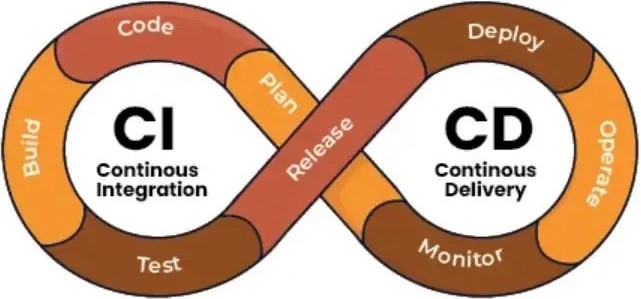
\includegraphics[width=0.55\linewidth]{img/02_wprowadzenie_teoretyczne/CI-CD.jpg}
  \caption{Przykład flow CI/CD \cite{geeksforgeeks_cicd}.}
\end{figure}

Typowy pipeline CI/CD składa się z następujących etapów:
\begin{enumerate}
  \item weryfikacja kodu (linting, testy jednostkowe),
  \item budowanie artefaktów (np. obrazu Docker),
  \item testy integracyjne i akceptacyjne,
  \item wdrożenie na środowisko docelowe,
  \item weryfikacja po wdrożeniu (smoke tests).
\end{enumerate}

\subsection{MLOps}

MLOps (ang. \textit{Machine Learning Operations}) to dyscyplina stosująca zasady DevOps do specyfiki cyklu życia modeli uczenia maszynowego. W odróżnieniu od klasycznego oprogramowania, gdzie artefaktem jest kod, w ML artefaktem jest model --- wynik trenowania na konkretnym zbiorze danych. To wprowadza kilka dodatkowych wyzwań:

\begin{itemize}
  \item dane treningowe zmieniają się niezależnie od kodu,
  \item wyniki trenowania są niedeterministyczne,
  \item jakość modelu musi być mierzona obiektywnie przed każdym wdrożeniem,
  \item modele degradują się w czasie (tzw. \textit{data drift}).
\end{itemize}

\begin{figure}[H]
  \centering
  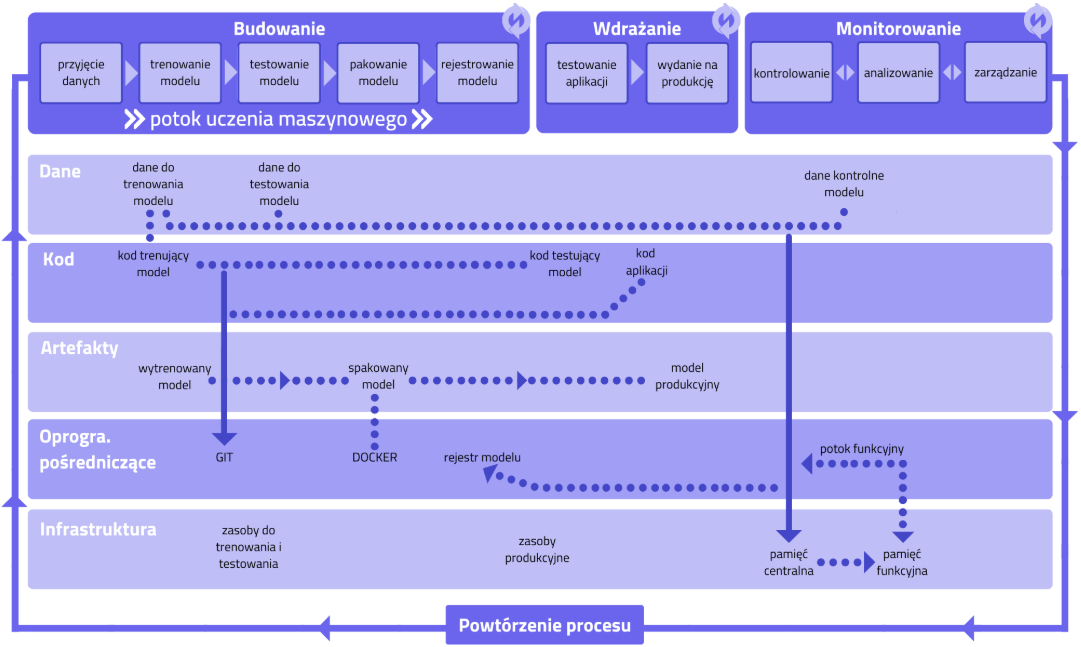
\includegraphics[width=\linewidth]{img/02_wprowadzenie_teoretyczne/mlops_flow.png}
  \caption{Przykład flow CI/CD \cite{mlops_flow}.}
\end{figure}

MLflow spina cały cykl życia modelu ML — od rejestrowania eksperymentów, parametrów i metryk podczas treningu, przez wersjonowanie oraz rejestrację modeli w Model Registry, aż po zarządzanie wdrożeniem i monitorowanie kolejnych wersji w środowisku produkcyjnym.
\subsection{Kontrola wersji --- Git i GitHub}

Git to rozproszony system kontroli wersji, będący de facto standardem w nowoczesnym tworzeniu oprogramowania \cite{chacon2014pro_git}. Przechowuje pełną historię zmian w postaci grafu migawek (ang. \textit{snapshots}), umożliwiając równoległą pracę na gałęziach (ang. \textit{branches}), scalanie zmian oraz cofanie się do dowolnego punktu w historii projektu.

Kluczowe koncepcje Gita:
\begin{itemize}
  \item \textbf{Commit} --- migawka stanu repozytorium w danym momencie wraz z metadanymi (autor, czas, wiadomość),
  \item \textbf{Branch} --- niezależna linia rozwoju; umożliwia pracę nad funkcjonalnością bez wpływu na gałąź główną,
  \item \textbf{Merge / Pull Request} --- scalenie zmian z jednej gałęzi do drugiej, zazwyczaj poprzedzone przeglądem kodu,
  \item \textbf{Hook} --- skrypt uruchamiany automatycznie w odpowiedzi na zdarzenie Gita (np. \texttt{pre-push}).
\end{itemize}

GitHub to platforma hostingowa dla repozytoriów Git, rozbudowana o funkcje współpracy zespołowej: pull requesty, przeglądy kodu, zarządzanie zadaniami oraz zintegrowane CI/CD w postaci GitHub Actions. W kontekście niniejszego projektu GitHub pełni rolę centralnego punktu integracji --- każda zmiana przechodzi przez repozytorium i może automatycznie uruchamiać kolejne etapy pipeline'u.

\subsection{GitHub Actions}

GitHub Actions to platforma automatyzacji wbudowana w GitHub, pozwalająca definiować przepływy pracy (ang. \textit{workflows}) jako pliki YAML przechowywane bezpośrednio w repozytorium \cite{github_actions_docs}. Workflow uruchamiane są w odpowiedzi na zdarzenia: push, pull request, harmonogram (cron) lub wywołanie ręczne.

Podstawowe pojęcia:
\begin{itemize}
  \item \textbf{Workflow} --- zestaw automatycznych zadań zdefiniowany w pliku \texttt{.github/workflows/*.yaml},
  \item \textbf{Job} --- jednostka wykonania złożona z kroków (steps); domyślnie uruchamiana równolegle z innymi jobami,
  \item \textbf{Step} --- pojedyncza operacja w ramach joba: wywołanie skryptu lub gotowej akcji,
  \item \textbf{Runner} --- maszyna wykonująca joba; może być zarządzana przez GitHub (hosted) lub przez użytkownika (self-hosted),
  \item \textbf{Artefakt} --- plik lub katalog przekazywany między jobami albo pobierany po zakończeniu workflow.
\end{itemize}

Kluczową cechą GitHub Actions jest możliwość użycia \textbf{self-hosted runners} --- maszyn zarządzanych przez użytkownika, co w niniejszym projekcie pozwala uruchamiać trening bezpośrednio na instancji EC2 wyposażonej w odpowiedni sprzęt obliczeniowy, bez potrzeby przekazywania danych treningowych przez sieć do zewnętrznego runnera.

\subsection{Konteneryzacja --- Docker}

Docker to platforma do tworzenia, dystrybucji i uruchamiania aplikacji w kontenerach \cite{merkel2014docker}. Kontener to izolowane środowisko uruchomieniowe zawierające aplikację wraz ze wszystkimi jej zależnościami: bibliotekami, interpreterem, zmiennymi środowiskowymi. Dzięki temu aplikacja działa identycznie na maszynie dewelopera, serwerze testowym i produkcji, eliminując problem \textit{,,u mnie działa''}.

Kluczowe pojęcia:
\begin{itemize}
  \item \textbf{Obraz (image)} --- niezmienialny szablon opisujący środowisko, definiowany plikiem \texttt{Dockerfile},
  \item \textbf{Kontener} --- działająca instancja obrazu; izolowana od systemu hosta i innych kontenerów,
  \item \textbf{Rejestr (registry)} --- repozytorium obrazów (np. Docker Hub, Amazon ECR).
\end{itemize}

W projekcie Docker służy do pakowania API modelu oraz do zapewnienia powtarzalności środowiska treningowego. Obraz z modelem jest budowany automatycznie w pipeline po zatwierdzeniu nowej wersji modelu.

\subsection{Kubernetes i k3s}

Kubernetes (K8s) to system do orkiestracji kontenerów --- automatyzuje ich wdrażanie, skalowanie i zarządzanie \cite{burns2016borg}. Zamiast uruchamiać kontenery ręcznie na konkretnych maszynach, Kubernetes przyjmuje deklaratywny opis pożądanego stanu (ile replik, jakie zasoby, jak reagować na awarie) i utrzymuje ten stan niezależnie od zdarzeń infrastrukturalnych.

k3s to uproszczona dystrybucja Kubernetes stworzona przez Rancher Labs. Zmniejsza wymagania sprzętowe (minimalna instalacja działa na instancji z 2~GB RAM) i upraszcza instalację do pojedynczego polecenia. Jest przeznaczona dla środowisk brzegowych, IoT oraz małych klastrów. W niniejszym projekcie k3s zainstalowany na pojedynczej instancji EC2 zastępuje zarządzany klaster EKS, co pozwala ograniczyć koszty do minimum.

\subsection{Infrastruktura jako kod --- Terraform i Helm}

\textbf{Infrastruktura jako kod} (ang. \textit{Infrastructure as Code}, IaC) to praktyka definiowania i zarządzania zasobami infrastrukturalnymi za pomocą plików konfiguracyjnych przechowywanych w systemie kontroli wersji, zamiast ręcznego konfigurowania przez interfejs graficzny lub CLI \cite{hashicorp_terraform}. Dzięki temu środowisko jest powtarzalne, audytowalne i odtwarzalne dowolnym momencie.

\textbf{Terraform} to narzędzie IaC firmy HashiCorp umożliwiające tworzenie, modyfikowanie i niszczenie zasobów chmurowych w deklaratywnym języku HCL (ang. \textit{HashiCorp Configuration Language}). Terraform utrzymuje plik stanu (\texttt{terraform.tfstate}) opisujący aktualną konfigurację infrastruktury, co pozwala wykrywać i stosować wyłącznie te zmiany, które są niezbędne. W projekcie Terraform zarządza zasobami AWS: siecią VPC, instancją EC2, zasobnikami S3 i rejestrem ECR.

\textbf{Helm} to menedżer pakietów dla Kubernetes, analogiczny do apt czy pip w świecie aplikacji \cite{helm_docs}. Pakiet Helm (ang. \textit{chart}) zawiera szablony zasobów Kubernetes parametryzowane wartościami z pliku \texttt{values.yaml}. Umożliwia to instalację, aktualizację i usuwanie złożonych aplikacji wieloskładnikowych jednym poleceniem, z pełną historią wdrożeń i możliwością cofnięcia (rollback). W projekcie Helm zarządza wdrożeniem API modelu oraz stosu monitorującego na klastrze k3s.

\subsection{Wersjonowanie danych --- DVC}

DVC (ang. \textit{Data Version Control}) to narzędzie umożliwiające wersjonowanie dużych plików binarnych (obrazów, wag modeli, zbiorów danych) w sposób spójny z Git. Zamiast przechowywać dane w repozytorium Git (co jest niepraktyczne przy dużych plikach), DVC przechowuje jedynie lekkie pliki metadanych (\texttt{.dvc}), a rzeczywiste dane trafiają do zewnętrznego magazynu --- w tym projekcie do Amazon S3 \cite{dvc_docs}.

Zasada działania jest analogiczna do Git: każda wersja danych ma swój hash, można cofać się do poprzednich wersji poleceniem \texttt{dvc checkout}, a polecenie \texttt{dvc pull} pobiera dane odpowiadające bieżącemu stanowi repozytorium. Dzięki temu możliwe jest odtworzenie dokładnego eksperymentu: tej samej wersji kodu, danych i konfiguracji.

\subsection{Śledzenie eksperymentów --- MLflow}

MLflow to platforma open-source do zarządzania cyklem życia modeli ML. Składa się z czterech głównych komponentów:

\begin{itemize}
  \item \textbf{Tracking} --- rejestrowanie parametrów, metryk i artefaktów każdego uruchomienia eksperymentu,
  \item \textbf{Projects} --- standaryzacja i reprodukowalność kodu ML,
  \item \textbf{Models} --- zunifikowany format pakowania modeli,
  \item \textbf{Model Registry} --- centralny rejestr wersji modeli z etapami cyklu życia (Staging, Production, Archived).
\end{itemize}

Model Registry jest kluczowym elementem w kontekście bramki jakości. Po każdym treningu nowa wersja modelu jest rejestrowana w MLflow. Bramka jakości pobiera metryki modelu aktualnie w etapie Production i porównuje z nowym wynikiem. Tylko model z lepszymi metrykami zostaje awansowany do Production \cite{mlflow_model_registry}.

\subsection{Monitoring --- Prometheus i Grafana}

Prometheus to system monitorowania i alertowania oparty na modelu \textit{pull} \cite{prometheus_docs}. Regularnie pobiera (ang. \textit{scrape}) metryki z endpointów HTTP udostępnianych przez monitorowane usługi i przechowuje je w wbudowanej bazie szeregów czasowych. Metryki opisywane są etykietami (ang. \textit{labels}), co pozwala na elastyczne filtrowanie i agregację.

Grafana to platforma wizualizacji danych, która integruje się z wieloma źródłami, w tym z Prometheus. Pozwala tworzyć interaktywne dashboardy z wykresami, wskaźnikami i alertami. W projekcie Grafana prezentuje metryki działającego API modelu: liczbę predykcji, czasy odpowiedzi, zużycie zasobów i liczbę błędów. Monitoring działa jako opcjonalny stos uruchamiany na tym samym klastrze k3s co API modelu \cite{grafana_intro}.
